\documentclass[10pt]{article}
\usepackage[margin=0.9in]{geometry}
\usepackage{graphicx}
\usepackage{booktabs}
\usepackage{amsmath}
\usepackage{float}
\usepackage[hidelinks]{hyperref}
\usepackage{caption}
\usepackage[numbers,sort&compress]{natbib}
\usepackage{microtype}
\graphicspath{{figures/}}
% Generated by scripts/exponential_bootstrap.py. Do not edit.
\newcommand{\betaSR}{0.382}
\newcommand{\sigSR}{0.028}
\newcommand{\nSR}{89}
\newcommand{\loSR}{0.322}
\newcommand{\hiSR}{0.432}
\newcommand{\betaQM}{0.327}
\newcommand{\sigQM}{0.016}
\newcommand{\nQM}{221}
\newcommand{\loQM}{0.286}
\newcommand{\hiQM}{0.349}
\newcommand{\betaEM}{0.325}
\newcommand{\sigEM}{0.010}
\newcommand{\nEM}{312}
\newcommand{\loEM}{0.313}
\newcommand{\hiEM}{0.353}
\newcommand{\betaWaves}{0.346}
\newcommand{\sigWaves}{0.017}
\newcommand{\nWaves}{126}
\newcommand{\loWaves}{0.303}
\newcommand{\hiWaves}{0.367}
\newcommand{\betaClassical}{0.360}
\newcommand{\sigClassical}{0.020}
\newcommand{\nClassical}{105}
\newcommand{\loClassical}{0.297}
\newcommand{\hiClassical}{0.377}
\newcommand{\betaThermo}{0.403}
\newcommand{\sigThermo}{0.021}
\newcommand{\nThermo}{73}
\newcommand{\loThermo}{0.371}
\newcommand{\hiThermo}{0.452}
\newcommand{\betaFluid}{0.422}
\newcommand{\sigFluid}{0.027}
\newcommand{\nFluid}{42}
\newcommand{\loFluid}{0.377}
\newcommand{\hiFluid}{0.483}
\newcommand{\simCrit}{3.45}
\newcommand{\nExclude}{0}
\newcommand{\bootN}{10000}
\newcommand{\bootSeed}{20261013}
\newcommand{\betaFeynBench}{0.342}
\newcommand{\sigFeynBench}{0.013}
\newcommand{\nFeynBench}{100}
\newcommand{\loFeynBench}{0.319}
\newcommand{\hiFeynBench}{0.371}
\newcommand{\betaFeynAll}{0.354}
\newcommand{\sigFeynAll}{0.008}
\newcommand{\nFeynAll}{1016}
\newcommand{\loFeynAll}{0.333}
\newcommand{\hiFeynAll}{0.366}
\newcommand{\betaWiki}{0.315}
\newcommand{\sigWiki}{0.015}
\newcommand{\nWiki}{76}
\newcommand{\loWiki}{0.284}
\newcommand{\hiWiki}{0.346}
\newcommand{\betaEI}{0.269}
\newcommand{\sigEI}{0.010}
\newcommand{\nEI}{70}
\newcommand{\loEI}{0.253}
\newcommand{\hiEI}{0.293}
\newcommand{\betaLeemis}{0.269}
\newcommand{\sigLeemis}{0.014}
\newcommand{\nLeemis}{61}
\newcommand{\loLeemis}{0.250}
\newcommand{\hiLeemis}{0.304}
\newcommand{\betafR}{0.270}
\newcommand{\sigfR}{0.021}
\newcommand{\nfR}{37}
\newcommand{\lofR}{0.264}
\newcommand{\hifR}{0.347}
\newcommand{\betaPooled}{0.354}
\newcommand{\sigPooled}{0.008}
\newcommand{\nPooled}{1016}
\newcommand{\nLabelled}{968}
\newcommand{\nFeynAllExpr}{1016}
\newcommand{\nLectAdded}{916}

% \input is not expandable inside tabular; the TeX primitive is.
\makeatletter\newcommand{\tabinput}[1]{\@@input #1 }\makeatother

\title{The grammar of physics is branch-dependent:\\ evidence from the Feynman Lectures}
% TODO(author): author name and affiliation (Chun Hin Ma?). Not filled in on purpose.
\author{}
\date{}

\begin{document}
\maketitle

\begin{center}
\fbox{\parbox{\dimexpr\linewidth-2\fboxsep-2\fboxrule\relax}{\centering
\emph{Working draft: this document is being actively edited and updated; numbers and text may change.}\par\medskip
Draft date: \today.
}}
\end{center}

\begin{abstract}
It has been reported~\citep{constantin2024} that operators in equations of physics, ranked by frequency, follow an exponential law $p_r\propto e^{-\beta r}$, with $\beta\approx0.34$ for the Feynman Lectures and Wikipedia but a lower value for the inflaton potentials of Encyclopaedia Inflationaris. We re-estimate $\beta$ by multinomial maximum likelihood, with bootstrap uncertainty over expressions, and confirm the gap: $\betaEI\pm\sigEI$ for Encyclopaedia Inflationaris against $\betaFeynBench\pm\sigFeynBench$ for the Feynman benchmark (likelihood ratio 38.9, permutation $p<0.00025$). We then test the explanations suggested for it in turn. Constant conventions do not account for it: natural units ($c=\hbar=1$) and setting the potentials' amplitude prefactor to one shift $\beta$ by at most 0.01 and widen rather than close the gap. Nor does the Lagrangian form of the potentials: ten $f(R)$ gravity Lagrangians give $\betafR\pm\sigfR$, in line with the textbook corpora, and random subsets of ten potentials rarely reach that value. The remaining suggestion, that the potentials describe a different physical regime, we recast as a question that can be tested within one source: does $\beta$ depend on the branch of physics? We extend the 100 expressions of the AI Feynman benchmark with every closed-form equation of the Feynman Lectures on Physics, Vol.~I--III, that sets a quantity equal to an expression built from nullary, unary and binary operators: \nFeynAll{} expressions after deduplication, \nLabelled{} of them assigned to seven branches by chapter. A shared $\beta$ is rejected (likelihood ratio \LRall{} on \dfall{} degrees of freedom, permutation $p<0.00025$, $\Delta\mathrm{AIC}=\dAICall$, $\Delta\mathrm{BIC}=\dBICall$). Against the other branches combined, quantum mechanics ($\betaQM\pm\sigQM$) lies below the rest, thermodynamics ($\betaThermo\pm\sigThermo$) and fluid and continuum mechanics ($\betaFluid\pm\sigFluid$) above it, and electromagnetism ($\betaEM\pm\sigEM$) slightly above it; special relativity ($\betaSR\pm\sigSR$, with relativistic electrodynamics chapters counted as relativity) is low before but not after multiple-comparison correction. The exponent of the rank law is therefore not one number for physics but depends on the branch.
\end{abstract}

\begin{figure}[h]\centering
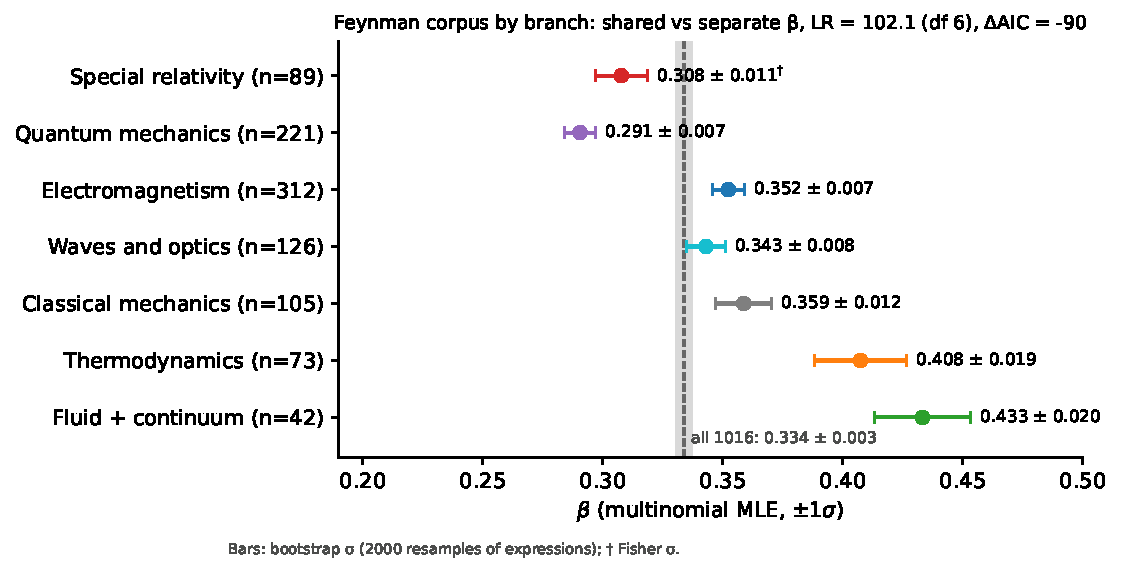
\includegraphics[width=0.8\linewidth]{beta_by_branch.pdf}
\caption{$\beta$ (multinomial MLE) for each branch of the Feynman corpus (AI Feynman benchmark plus the Feynman Lectures Vol.~I--III, deduplicated). Bars are $\pm1\sigma$: bootstrap over expressions, except special relativity (Fisher $\sigma$, marked $\dagger$; Section~\ref{sec:methods}). The dashed line and grey band are all \nPooled{} expressions pooled, $\betaPooled\pm\sigPooled$.}\label{fig:main}
\end{figure}

\section{Introduction}
Previous work~\citep{constantin2024} represents each equation of physics as an expression tree and counts its operators: nullary operators (variables, constants, numbers), unary operators (such as $\sin$, $\exp$, $\sqrt{\cdot}$) and binary operators ($+$, $-$, $\times$, $\div$, powers). Summing counts over a corpus and ranking operator types by frequency yields an exponentially decaying frequency at rank $r$,
\begin{equation}
p_r(\beta) = \frac{e^{-\beta r}}{\sum_{s=1}^{R} e^{-\beta s}},\qquad r=1,\dots,R,
\label{eq:law}
\end{equation}
where $R$ is the number of operator types that occur. Using simulation-based inference, that study reports $\beta=0.342\pm0.010$ for 100 expressions from the Feynman Lectures (the AI Feynman benchmark~\citep{udrescu2020}), $0.35\pm0.03$ for equations from Wikipedia, and a lower $0.266\pm0.014$ for the inflaton potentials of Encyclopaedia Inflationaris~\citep{martin2014}, and interprets the exponential law with a characteristic $\beta$ as a statistical regularity of how physics is written.

The lower value for Encyclopaedia Inflationaris is the puzzle we start from. Several accounts of it are possible: the conventions for constants (natural units, and an energy-density prefactor shared by all potentials); the form of the expressions (the potentials enter a Lagrangian, and are many candidate expressions for one concept in a theory that is not established); and a different energy scale or physical regime from that of the textbook equations. We address them in this order. The first two can be tested directly, by rewriting the expressions and by measuring a comparable corpus of Lagrangians. The third cannot be tested on Encyclopaedia Inflationaris alone, so we recast it as a question that can be answered within one source: if $\beta$ depends on the regime an equation describes, it should differ between branches of physics written by the same author. The published corpora are not suited to that test: the 100 benchmark expressions span seven branches but provide only 2--33 expressions per branch, too few to resolve $\beta$ values that differ by a few hundredths, and cross-source comparisons would confound branch with notation and editorial convention. We therefore assemble a single-source corpus large enough to resolve branches: every closed-form equation of the Feynman Lectures on Physics~\citep{feynman} satisfying the selection rule of Section~\ref{sec:data}, together with the benchmark.

Our contributions follow this argument:
\begin{enumerate}
\item a re-estimation of $\beta$ for Encyclopaedia Inflationaris and five other corpora with one likelihood-based estimator, confirming the lower value (Section~\ref{sec:corpora});
\item tests of the constant conventions---natural units and the amplitude prefactor---which do not close the gap (Section~\ref{sec:units});
\item a test of the Lagrangian form with ten $f(R)$ Lagrangians, which do not reproduce the low value (Section~\ref{sec:fr});
\item a catalog of \nFeynAll{} deduplicated Feynman expressions with operator counts, chapter-level branch labels and source links (Section~\ref{sec:data}), and a likelihood-ratio test, calibrated by permutation, of a shared $\beta$ against branch-specific values, which finds that $\beta$ depends on the branch of physics (Section~\ref{sec:results}).
\end{enumerate}

\section{Data}\label{sec:data}

\subsection{Corpora}
\begin{description}
\item[Feynman benchmark.] The 100 expressions of the AI Feynman benchmark~\citep{udrescu2020} as released with~\citep{constantin2024}, each traced to a chapter of the Feynman Lectures. Each carries a branch label.
\item[Feynman Lectures, Vol.~I--III.] Expressions extracted from the online edition~\citep{feynman} (below): 309 from Vol.~I, 487 from Vol.~II and 216 from Vol.~III after the manual recheck.
\item[Wikipedia.] The 41 released expressions from the list of equations named after people~\citep{wikinamed}, and the 35 added after the release cutoff in the same list (\nWiki{} in total).
\item[Encyclopaedia Inflationaris (EI).] The \nEI{} released inflaton potentials~\citep{martin2014}.
\item[Leemis.] The \nLeemis{} probability density functions of the univariate distribution chart~\citep{leemis2008} that satisfy the selection rule; a corpus of mathematics rather than physics.
\item[$f(R)$.] Ten closed forms of $f(R)$ from the modified-gravity literature~\citep{sotiriou2010}: candidate expressions for one function in the gravitational action.
\end{description}

\subsection{Selection rule}
An equation is retained if it equates a single quantity to a closed-form expression whose operators are nullary (variables, named physical constants, numbers), unary or binary; operator counts refer to the right-hand side. Equations are excluded if the left-hand side is not a single plain quantity (e.g.\ vector components written as products, derivatives, or multiple quantities), if the right-hand side contains a derivative, integral, sum, limit, operator hat or complex conjugate, if it is trivial (a single symbol or number), or if it lacks an equals sign. Physical constants ($c$, $\hbar$, $h$, $G$, $k_B$, $\epsilon_0$, $\mu_0$, $e$, \dots) are counted as constants, not variables. Powers $x^2$, $x^3$ and $x^4$ are each counted as one unary operator, following the upstream convention~\citep{constantin2024}.

\subsection{Extraction from the Feynman Lectures}
The online Feynman Lectures embed equations as \LaTeX{} source rendered by MathJax. From the chapter HTML (Vol.~I chapters 1--52, Vol.~II 1--42, Vol.~III 1--21) we extract every display equation, expand page-level macros, split aligned environments into rows, attach continuation rows (\texttt{\&=}) to their left-hand side, and record the equation number. Duplicate renderings of the same equation (wide and narrow layouts) are dropped. Each row is filtered by the selection rule, parsed from \LaTeX{} into a symbolic expression, and counted with the same pipeline as the other corpora. Of 4{,}980 display equations, the automatic pipeline retains 1{,}063 (Vol.~I 311 of 1{,}152; Vol.~II 502 of 2{,}195; Vol.~III 250 of 1{,}633). After the manual recheck below, 1{,}012 remain (Vol.~I 309, Vol.~II 487, Vol.~III 216). Each record stores volume, chapter, section, equation number and a link to the equation on the Caltech site.

\paragraph{Deduplication.} A Lectures record is dropped if it is one of the 100 benchmark expressions (63 records, matched by equation number or, failing that, by chapter and operator signature), if it has the same chapter, operator shape and constants as a benchmark expression (9), or if it is symbolically identical to an earlier record (24). This leaves \nLectAdded{} Lectures expressions and a Feynman corpus of \nFeynAll{}.

\paragraph{Quality assurance.} After two rounds of sampled checks, we compared all 1{,}063 retained records by hand to the source \LaTeX{}. The recheck altered 83 records (Table~\ref{tab:recheck}): 51 were rejected and 32 corrected. The most frequent issues were amplitude brackets $\langle a|b\rangle$ on the right-hand side (25 records, all Vol.~III), which the parser had collapsed to single symbols, and function notation such as $J(t-x/c)$ or $\cos\omega(t-r/c)$ parsed as products (13). Corrections are applied post hoc from a tracked file, \texttt{data/feynman\_lectures\_fixes.csv}, listing for each changed record the action, error type, revised expression and reason; corrected catalog entries retain the prior expression. Time averages $\langle x\rangle$ of a physical quantity are retained as one symbol; $q_e$ is counted as a variable, as in the benchmark.

\begin{table}[H]\centering\small
\begin{tabular}{lrrrr}\toprule
Error type & Vol.~I & Vol.~II & Vol.~III & Action\\\midrule
Amplitude brackets on the right-hand side & -- & -- & 25 & reject\\
Operator or matrix expression & -- & -- & 5 & reject\\
Left-hand side not one quantity & 1 & 4 & 3 & reject\\
Function value parsed as a product & 4 & 7 & 2 & 2 reject, 11 fix\\
Truncated aligned row & 1 & 3 & -- & reject\\
Implicit equation (quantity on both sides) & -- & 3 & -- & reject\\
Numerical value with unit text & -- & 4 & -- & 2 reject, 2 fix\\
Special function or derivative notation & -- & 2 & -- & reject\\
Other parse error (macro, lost subscript, wrong row) & 4 & 3 & 4 & fix\\
Sign artefact ($-1\times$) & 2 & -- & -- & fix\\
Symbol name only (counts unchanged) & -- & 1 & 3 & fix\\
Constant counted as a variable ($\kappa$ for $k_B$) & -- & -- & 2 & fix\\\midrule
Total & 12 & 27 & 44 & 51 reject, 32 fix\\\bottomrule
\end{tabular}
\caption{Changes from the full recheck of the Feynman Lectures records against the source \LaTeX{}.}\label{tab:recheck}
\end{table}

\subsection{Branches}
Each Lectures chapter is assigned to one branch (classical mechanics, special relativity, electromagnetism, waves and optics, thermodynamics and kinetic theory, quantum mechanics, fluid mechanics, continuum mechanics) or to a label excluded from the branch test (mathematics, probability, general relativity, overview chapters); benchmark expressions retain their published labels. Fluid and continuum mechanics are merged (10 and 32 expressions). Relativistic electrodynamics (Vol.~I ch.~34; Vol.~II ch.~25, 26 and 28) is coded as special relativity, as is the single benchmark expression labelled electromagnetism from those chapters (Vol.~I ch.~34). Of the \nFeynAll{} expressions, \nLabelled{} lie in the seven test branches; the remaining 48 are mathematics (31), probability (9), general relativity (6) and two unassigned.

\section{Methods}\label{sec:methods}

\paragraph{What $\beta$ is.} For a group of expressions, count how often each operator type appears (each variable, constant, number, $\sin$, $+$, $\times$, \dots{} counts as one instance) and rank types from most to least frequent. The parameter $\beta$ governs how rapidly frequencies decay with rank: by Eq.~\eqref{eq:law}, each step down the ranking multiplies the expected frequency by $e^{-\beta}$. At $\beta=0.34$, each rank carries roughly 71\% of the frequency of the preceding rank; larger $\beta$ concentrates usage on fewer operator types, smaller $\beta$ spreads it more evenly.

\paragraph{Estimator.} We estimate $\beta$ by maximum likelihood under a multinomial model. Sum the operator counts of the group, sort the $R$ operator types that occur by count, $n_1\ge n_2\ge\dots\ge n_R$, and treat each of the $N=\sum_r n_r$ operator instances as an independent draw that lands on rank $r$ with probability $p_r(\beta)$ from Eq.~\eqref{eq:law}. The probability of the observed counts is then multinomial, $P(n_1,\dots,n_R\mid\beta)=\frac{N!}{\prod_r n_r!}\prod_r p_r(\beta)^{n_r}$, and the log-likelihood, up to a term that does not depend on $\beta$, is
\begin{equation}
\ell(\beta) = \sum_{r=1}^{R} n_r \log p_r(\beta) = -\beta\sum_r r\,n_r - N\log\sum_{s=1}^{R}e^{-\beta s},
\end{equation}
and $\hat\beta$ maximises $\ell$ (bounded scalar optimisation on $[0,5]$). Setting $d\ell/d\beta=0$ shows that the estimate is the $\beta$ for which the model mean rank of an operator instance equals the observed mean rank, $\sum_r r\,n_r/N$. Unlike a linear fit to $\log n_r$ versus $r$, the likelihood weights each rank by its instance count, so sparse tail ranks with one or two instances carry little weight.

\paragraph{Uncertainty.} Uncertainty is estimated by bootstrapping over expressions rather than operator instances, because instances within a single expression are not independent. For each group we resample expressions with replacement (2{,}000 replicates, seed 20261013), sum counts, re-rank operator types and refit; the standard deviation across replicates is the bootstrap $\sigma$. Re-ranking is essential, since which operator occupies rank 3 can change between replicates. We also report the Fisher error $\sigma_F = [N\,\mathrm{Var}_{p(\hat\beta)}(r)]^{-1/2}$, which treats instances as independent. In the main analysis the two agree to within 0.004 for every branch. We quote the Fisher $\sigma$ for special relativity and the bootstrap $\sigma$ elsewhere: without the relativistic electrodynamics chapters, special relativity would have 32 expressions over only 9 ranks, with a few long expressions dominating the instance count, and its bootstrap distribution becomes skewed, so we use the Fisher value for this branch throughout.

\paragraph{Tests.} For $G$ groups we compare a shared model (one $\beta$, ranks computed within each group) to separate $\beta_g$ via the likelihood ratio $\Lambda = 2(\ell_{\text{sep}}-\ell_{\text{shared}})$ on $G-1$ degrees of freedom. Because the $\chi^2$ reference assumes independent operator instances, we calibrate $\Lambda$ by permutation: expressions are shuffled among groups of the observed sizes and $\Lambda$ recomputed \permreps{} times; $p=(k+1)/(\permreps+1)$, where $k$ counts permutations at least as extreme (smallest attainable $p=1/4001\approx0.00025$). We report $\Delta\mathrm{AIC}$ and $\Delta\mathrm{BIC}$ (separate minus shared; negative values favour separate $\beta$), with $N$ the operator-instance count in the BIC.

We consider three test families: all seven branches jointly; each branch against the other six pooled (Bonferroni factor 7); and all 21 pairwise branch comparisons (Bonferroni factor 21).

\paragraph{Power.} The minimum detectable pairwise difference in $\beta$ at $\alpha=0.05$ and 80\% power is $(z_{0.975}+z_{0.8})\sqrt{\sigma_a^2+\sigma_b^2}$. We additionally simulate multinomial counts at the observed $N$ and $R$ for a branch and the pooled remainder, with the branch $\beta$ shifted by $\Delta\beta$, and record the fraction of $\chi^2$ likelihood-ratio tests rejecting at 5\% (1{,}000 simulations per point; $N$ deflated by the squared bootstrap-to-Fisher $\sigma$ ratio when that ratio exceeds one).

\section{The lower \texorpdfstring{$\beta$}{beta} of Encyclopaedia Inflationaris}\label{sec:ei}

\subsection{\texorpdfstring{$\beta$}{beta} by corpus}\label{sec:corpora}
Table~\ref{tab:corpus} and Figure~\ref{fig:corpus} compare corpora using the same estimator. The Feynman benchmark, full Feynman corpus, Wikipedia and $f(R)$ are mutually consistent ($\beta$ in the range 0.334--0.346). Encyclopaedia Inflationaris is lower: $\betaEI\pm\sigEI$ vs.\ $\betaFeynBench\pm\sigFeynBench$ for the benchmark ($\Lambda=38.9$, df 1, permutation $p<0.00025$, $\Delta\mathrm{AIC}=-37$, $\Delta\mathrm{BIC}=-31$). Leemis, a corpus of probability densities rather than physics, falls between them ($\betaLeemis\pm\sigLeemis$).

\begin{table}[H]\centering\small
\begin{tabular}{lrrrrr}\toprule
Corpus & Expr. & Instances & $\hat\beta$ & Boot.\ $\sigma$ & Fisher $\sigma$\\\midrule
\tabinput{generated/corpus_table.tex}
\bottomrule
\end{tabular}
\caption{$\beta$ by corpus (multinomial MLE; bootstrap 2{,}000 replicates).}\label{tab:corpus}
\end{table}

\begin{figure}[H]\centering
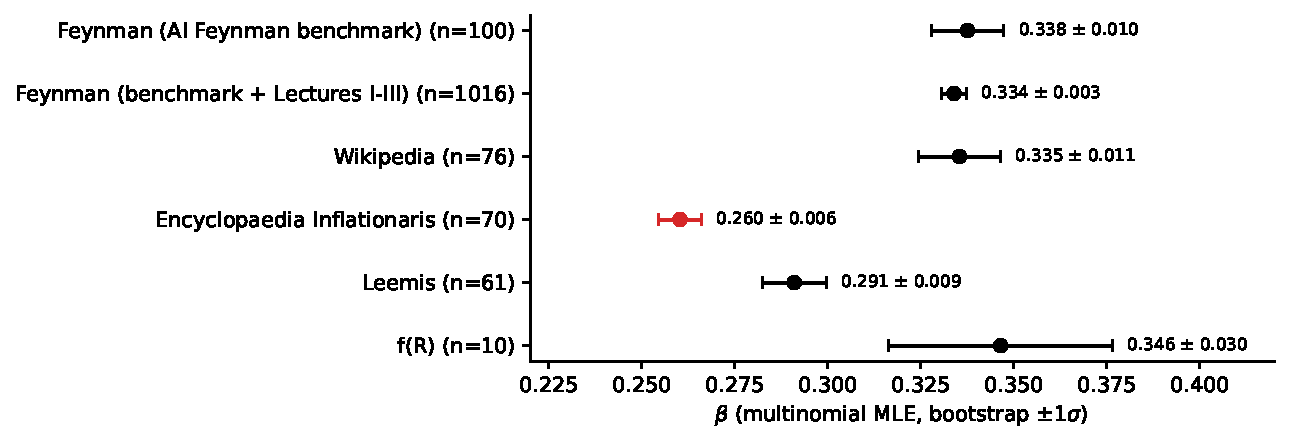
\includegraphics[width=0.75\linewidth]{beta_by_corpus.pdf}
\caption{$\beta$ by corpus, bootstrap $\pm1\sigma$. Encyclopaedia Inflationaris in red.}\label{fig:corpus}
\end{figure}

\subsection{Constant conventions}\label{sec:units}
Encyclopaedia Inflationaris writes its potentials in natural units, and every potential carries an energy-density prefactor $M^4$, whereas the textbook corpora keep $c$, $\hbar$ and other constants explicit. Both conventions change the operator counts. Rewriting the Feynman benchmark with $c=\hbar=1$ (32 expressions affected) shifts its $\beta$ from 0.338 to $0.348\pm0.011$, and Wikipedia (2 affected) from 0.335 to $0.336\pm0.011$; setting $M=1$ in all 70 potentials moves Encyclopaedia Inflationaris from 0.260 to $0.257\pm0.006$ (\texttt{results/units\_check.json}). Each rewrite changes $\beta$ by at most 0.01, and the benchmark--EI gap widens rather than closes. The conventions for constants do not explain the lower value.

\subsection{Lagrangian form: \texorpdfstring{$f(R)$}{f(R)} gravity}\label{sec:fr}
The inflaton potentials are terms in a Lagrangian rather than equations for a measured quantity, and they are many candidate expressions for one concept in a theory that is not established. Ten closed forms of $f(R)$, the function that replaces the Ricci scalar in the Einstein--Hilbert action~\citep{sotiriou2010}, share all three properties. They give $\betafR\pm\sigfR$, in line with the textbook corpora (Table~\ref{tab:corpus}). Because this corpus is small, we compare it with subsets of the same size: 2{,}000 random subsets of 10 Encyclopaedia Inflationaris potentials (seed 20260930) have median $\beta=0.257$ (16--84\%: 0.242--0.273, maximum 0.312; \texttt{results/ei\_sample10.json}), so a corpus of ten potentials rarely reaches the $f(R)$ value (Figure~\ref{fig:ei}). Being a Lagrangian, or a set of candidates for one unproven concept, does not by itself produce a low $\beta$.

\begin{figure}[H]\centering
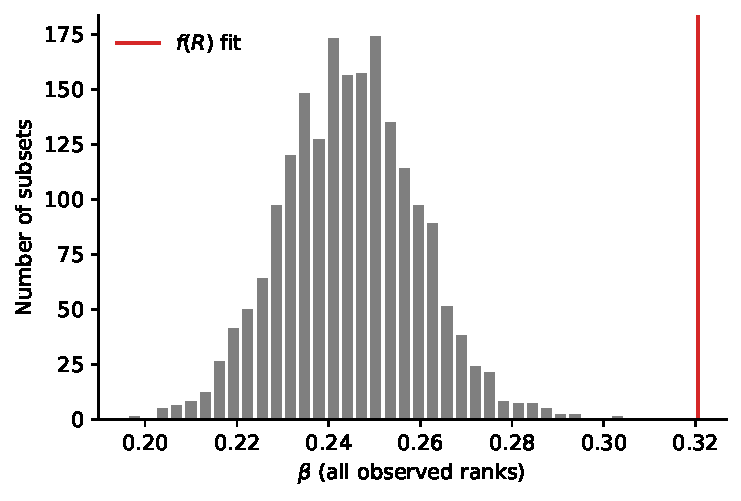
\includegraphics[width=0.5\linewidth]{ei_sample10_beta.pdf}
\caption{$\beta$ of 2{,}000 random subsets of 10 Encyclopaedia Inflationaris potentials.}\label{fig:ei}
\end{figure}

The remaining account is that the potentials describe a different energy scale or physical regime. Encyclopaedia Inflationaris offers no second regime to compare with, but the question has a testable form within a single source: whether $\beta$ depends on the branch of physics an equation belongs to. Section~\ref{sec:results} answers it.

\section{Branch dependence within the Feynman Lectures}\label{sec:results}

\subsection{\texorpdfstring{$\beta$}{beta} by branch}
Table~\ref{tab:branch} and Figure~\ref{fig:main} report $\hat\beta$ by branch. Figure~\ref{fig:rf} plots rank-frequency data with fitted exponentials: the law fits each branch reasonably well, with the largest residuals in the sparse highest ranks.

\begin{table}[H]\centering\small
\resizebox{\linewidth}{!}{\begin{tabular}{lrrrrrrrr}\toprule
Branch & Expr. & Instances $N$ & Ranks $R$ & $\hat\beta$ & Boot.\ $\sigma$ & Fisher $\sigma$ & Quoted $\sigma$ & $p$ vs rest (Bonf.)\\\midrule
\tabinput{generated/branch_table.tex}
\midrule
All Feynman expressions & \nPooled & 10693 & & \betaPooled & \sigPooled & 0.003 & \sigPooled & \\\bottomrule
\end{tabular}}
\caption{$\beta$ by branch, Feynman corpus. Last column: permutation $p$ of the branch against the other six pooled, times 7 (Bonferroni); ``$<$'' means no permutation was as extreme. $^a$Fisher $\sigma$ quoted (Section~\ref{sec:methods}).}\label{tab:branch}
\end{table}

\begin{figure}[H]\centering
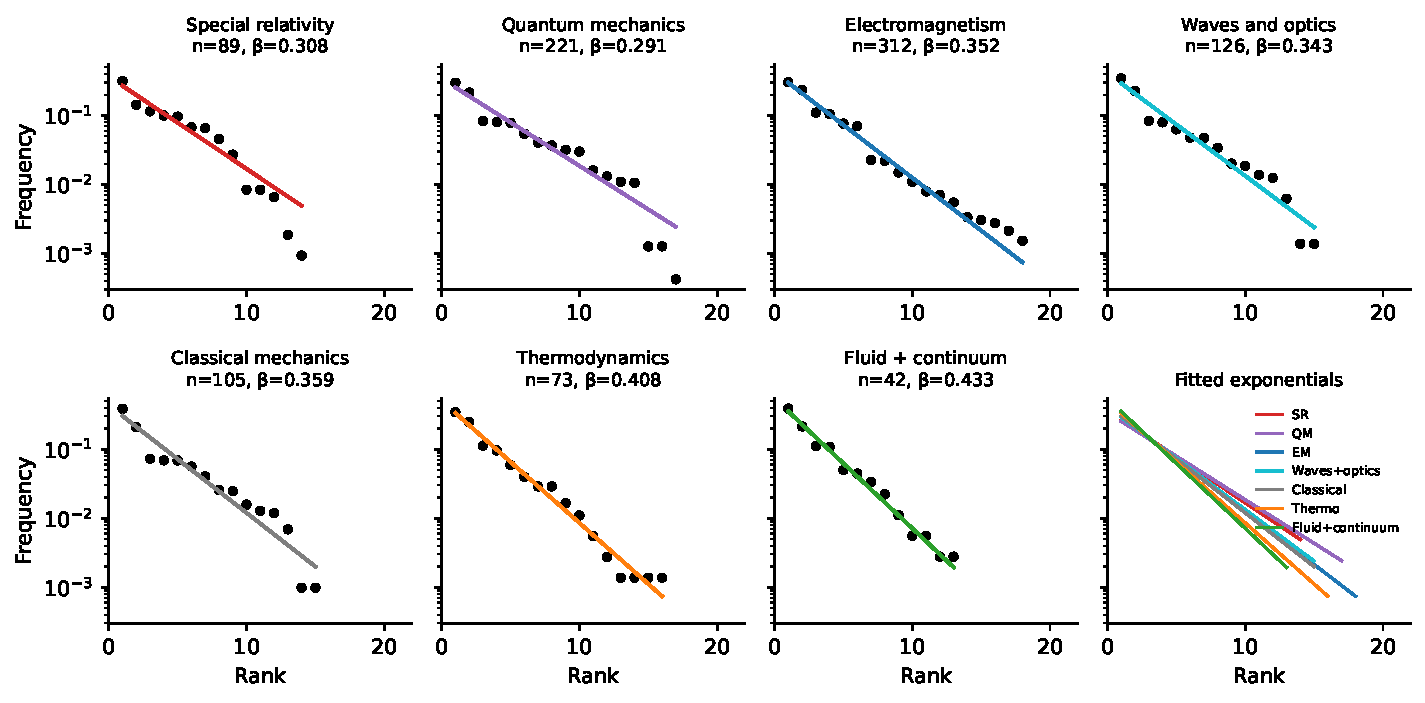
\includegraphics[width=\linewidth]{rank_frequency_branches.pdf}
\caption{Rank-frequency of operator instances in each branch (points) and the fitted exponential (line). Last panel: the seven fitted laws together.}\label{fig:rf}
\end{figure}

\subsection{Shared versus separate \texorpdfstring{$\beta$}{beta}}
Branch-specific $\beta$ fits substantially better than a single shared value: $\Lambda=\LRall$ on \dfall{} degrees of freedom ($\chi^2$ $p=\pchiall$; permutation $p<0.00025$, with none of \permreps{} permutations as extreme), $\Delta\mathrm{AIC}=\dAICall$, $\Delta\mathrm{BIC}=\dBICall$. Coarser grouping into five branches (classical mechanics with special relativity; electromagnetism with waves and optics) yields the same conclusion ($\Lambda=93.3$, df 4, permutation $p<0.00025$, $\Delta\mathrm{AIC}=-85$).

After Bonferroni correction (Table~\ref{tab:branch}), four branches differ from the pooled remainder: quantum mechanics is lower; thermodynamics, fluid and continuum mechanics, and---by a smaller margin---electromagnetism ($0.352$ vs.\ $0.325$ for the rest, $\Lambda=13.8$) are higher. Special relativity is low before correction ($p=0.0075$) but not after ($p=0.05$). Waves and optics ($p=1.00$ corrected) and classical mechanics ($p=0.23$ corrected) are consistent with the remainder.

Table~\ref{tab:pairs} lists uncorrected pairwise permutation $p$-values. Electromagnetism, waves and optics and classical mechanics cluster together (pairwise $p$ between 0.24 and 0.64), as do thermodynamics and fluid and continuum mechanics ($p=0.39$) and special relativity with quantum mechanics ($p=0.14$). Special relativity differs from classical mechanics before correction ($p=0.0035$; $\Lambda=9.7$, $\Delta\mathrm{AIC}=-7.7$). Under the $\times21$ correction (threshold $0.05/21\approx0.0024$), quantum mechanics differs from every branch except special relativity; special relativity differs from electromagnetism, thermodynamics and fluid and continuum mechanics; electromagnetism, waves and optics and classical mechanics each differ from fluid and continuum mechanics; and electromagnetism and waves and optics differ from thermodynamics. Classical mechanics vs.\ thermodynamics ($p=0.0085$ uncorrected), special relativity vs.\ waves and optics ($p=0.0090$) and special relativity vs.\ classical mechanics ($p=0.0035$) do not survive correction.

\begin{table}[H]\centering\small
\begin{tabular}{lccccccc}\toprule
 & SR & QM & EM & Waves & Classical & Thermo & Fluid\\\midrule
\tabinput{generated/pairwise_table.tex}
\bottomrule
\end{tabular}
\caption{Pairwise permutation $p$-values (\permreps{} permutations, uncorrected). ``$<0.0002$'' means no permutation was as extreme ($p\le1/4001$).}\label{tab:pairs}
\end{table}

\paragraph{Power.} The minimum detectable pairwise difference (80\% power, $\alpha=0.05$) is 0.026--0.029 among electromagnetism, quantum mechanics and waves and optics; 0.036--0.045 for pairs involving special relativity or classical mechanics with those branches; and 0.057--0.078 for pairs with thermodynamics or fluid and continuum mechanics. For $\Delta\beta=0.04$ against the remainder, simulated power is $\ge 0.99$ for quantum mechanics and electromagnetism, 0.96 for waves and optics, 0.89 for classical mechanics, 0.79 for special relativity, and 0.55 and 0.42 for thermodynamics and fluid and continuum mechanics. Non-rejections for waves and optics and classical mechanics are therefore informative at the $\sim 0.03$--$0.04$ scale: deviations of that magnitude would likely have been detected. The full grid is in \texttt{results/branch\_test.json}.

\section{Discussion}\label{sec:discussion}

\paragraph{Small branches.} The quoted Fisher $\sigma$ for special relativity treats operator instances as independent and may be too small. Permutation $p$-values do not rely on either uncertainty estimate. Fluid and continuum mechanics (42 expressions) and thermodynamics (73) are likewise small; power to detect a difference of 0.04 from the rest is about one half for them.

\paragraph{Extraction errors.} All retained records were hand-checked against source \LaTeX{}; 83 of 1{,}063 were rejected or corrected (Section~\ref{sec:data}). Subtle mis-parses may remain (e.g.\ a dropped prime or mis-read index with negligible count change). Before recheck, errors concentrated in Vol.~III (44 of 250 records changed, vs.\ 12 of 311 in Vol.~I and 27 of 502 in Vol.~II); recheck moved the quantum-mechanics $\beta$ from 0.300 to 0.291.

\paragraph{Scope.} All expressions derive from one textbook series and its benchmark subset. The results show that $\beta$ varies across branches \emph{as represented in the Feynman Lectures}; generalisation to other texts is untested. Counts follow conventions aligned with~\citep{constantin2024} (constants vs.\ variables; powers $x^2$--$x^4$ as unary operators), and the selection rule omits differential and integral equations, which dominate much of the subject matter in every branch.

\section{Conclusion}
The lower $\beta$ of Encyclopaedia Inflationaris is confirmed with a likelihood-based estimator, and two suggested explanations are ruled out: rewriting the constants (natural units, the amplitude prefactor) changes $\beta$ by at most 0.01 and widens the gap, and a corpus of $f(R)$ Lagrangians, also candidates for one unproven concept, has the textbook value. Recast as a question about physical regime, the remaining explanation is supported within a single source: in the Feynman Lectures plus the AI Feynman benchmark, the exponential rank law for operator frequencies holds in each branch, but a common $\beta$ is strongly rejected. Thermodynamics and fluid and continuum mechanics lie above electromagnetism, waves and optics and classical mechanics, and quantum mechanics lies below them. A single $\beta$ for ``physics'' is thus an average over branches whose estimates differ by up to 0.14, and a corpus drawn from one subject, such as inflaton potentials, need not share the textbook value.

\bibliographystyle{unsrtnat}
\bibliography{refs}
\end{document}
